\subsection{Condition-Level Performance}
Table~\ref{tab:condition_summary} presents condition-level performance across 30 Gazebo simulation runs ($n=3$ per condition, reporting mean $\pm$ sample standard deviation with Bessel correction $ddof=1$). All 10 conditions achieved a $100\%$ replay audit pass rate ($3/3$), confirming physical halt stability and data completeness across all runs.

\begin{table*}[t]
\centering
\caption{Condition-Level Navigation Performance Across 30 Gazebo Simulation Runs ($n=3$ per condition, mean $\pm$ sample std dev, $ddof=1$).}
\label{tab:condition_summary}
\resizebox{\textwidth}{!}{%
\begin{tabular}{llclcccccc}
\hline
Scenario & Method & $n$ & Actual Route & Dead-Ends & Decision Dist (m) & Decision Time (s) & Total Dist (m) & Total Time (s) & Replay Audit Pass \\
\hline
D0 & R & 3 & Path\_A & 0.0 $\pm$ 0.0 & 6.16 $\pm$ 0.04 & 51.5 $\pm$ 1.7 & 6.16 $\pm$ 0.04 & 51.5 $\pm$ 1.7 & 3/3 (100\%) \\
D0 & O & 3 & Path\_A & 0.0 $\pm$ 0.0 & 6.20 $\pm$ 0.01 & 50.0 $\pm$ 0.8 & 6.20 $\pm$ 0.01 & 50.0 $\pm$ 0.8 & 3/3 (100\%) \\
D0 & F & 3 & Path\_A & 0.0 $\pm$ 0.0 & 6.20 $\pm$ 0.03 & 49.9 $\pm$ 0.5 & 6.20 $\pm$ 0.03 & 49.9 $\pm$ 0.5 & 3/3 (100\%) \\
D1 & R & 3 & Path\_A\_then\_Path\_B & 1.0 $\pm$ 0.0 & 10.82 $\pm$ 0.07 & 82.1 $\pm$ 4.4 & 17.22 $\pm$ 0.24 & 141.0 $\pm$ 5.9 & 3/3 (100\%) \\
D1 & O & 3 & Path\_B & 0.0 $\pm$ 0.0 & 7.55 $\pm$ 0.05 & 50.0 $\pm$ 2.0 & 13.95 $\pm$ 0.07 & 108.7 $\pm$ 2.7 & 3/3 (100\%) \\
D1 & F & 3 & Path\_B & 0.0 $\pm$ 0.0 & 7.54 $\pm$ 0.00 & 48.2 $\pm$ 1.0 & 14.03 $\pm$ 0.25 & 109.5 $\pm$ 1.6 & 3/3 (100\%) \\
D2 & R & 3 & Path\_A & 0.0 $\pm$ 0.0 & 5.92 $\pm$ 0.04 & 49.6 $\pm$ 1.6 & 16.34 $\pm$ 0.03 & 148.2 $\pm$ 3.2 & 3/3 (100\%) \\
D2 & O & 3 & Path\_A & 0.0 $\pm$ 0.0 & 5.94 $\pm$ 0.07 & 52.0 $\pm$ 1.7 & 16.40 $\pm$ 0.24 & 149.8 $\pm$ 0.6 & 3/3 (100\%) \\
D2 & F & 3 & Path\_A & 0.0 $\pm$ 0.0 & 5.89 $\pm$ 0.02 & 51.1 $\pm$ 1.0 & 16.25 $\pm$ 0.10 & 151.1 $\pm$ 7.8 & 3/3 (100\%) \\
D2 & M1 & 3 & Path\_B & 0.0 $\pm$ 0.0 & 7.89 $\pm$ 0.02 & 51.3 $\pm$ 2.0 & 18.25 $\pm$ 0.09 & 148.8 $\pm$ 2.4 & 3/3 (100\%) \\
\hline
\end{tabular}%
}
\end{table*}


\subsection{Pairwise Contrasts \& Trajectory Analysis}
Table~\ref{tab:pairwise_contrasts} reports pairwise contrast comparisons across evaluated methods, and Figure~\ref{fig:trajectories} illustrates representative trajectories from the Gazebo simulation runs.

\begin{table}[t]
\centering
\footnotesize
\caption{Key Pairwise Contrasts Between Methods Across Scenarios D1 and D2.}
\label{tab:pairwise_contrasts}
\setlength{\tabcolsep}{2.5pt}
\begin{tabular}{lllcccc}
\toprule
Scenario & Contrast & Metric & $A$ & $B$ & \shortstack{Diff\\($A-B$)} & \shortstack{Rel\\(\%)} \\
\midrule
D1 & $F$ vs. $R$  & Dist (m) & 14.03  & 17.22  & -3.19  & -18.5\% \\
D1 & $F$ vs. $R$  & Time (s) & 109.50 & 141.00 & -31.50 & -22.3\% \\
D1 & $O$ vs. $R$  & Dist (m) & 13.95  & 17.22  & -3.27  & -19.0\% \\
D1 & $O$ vs. $R$  & Time (s) & 108.70 & 141.00 & -32.30 & -22.9\% \\
D1 & $F$ vs. $O$  & Dist (m) & 14.03  & 13.95  & +0.08  & +0.6\%  \\
D1 & $F$ vs. $O$  & Time (s) & 109.50 & 108.70 & +0.80  & +0.7\%  \\
D2 & $F$ vs. $M1$ & Dist (m) & 16.25  & 18.25  & -2.00  & -11.0\% \\
D2 & $F$ vs. $M1$ & Time (s) & 151.10 & 148.83 & +2.27  & +1.5\%  \\
D2 & $F$ vs. $O$  & Dist (m) & 16.25  & 16.40  & -0.15  & -0.9\%  \\
D2 & $F$ vs. $O$  & Time (s) & 151.10 & 149.77 & +1.33  & +0.9\%  \\
\bottomrule
\end{tabular}
\end{table}


\begin{figure}[t]
\centering
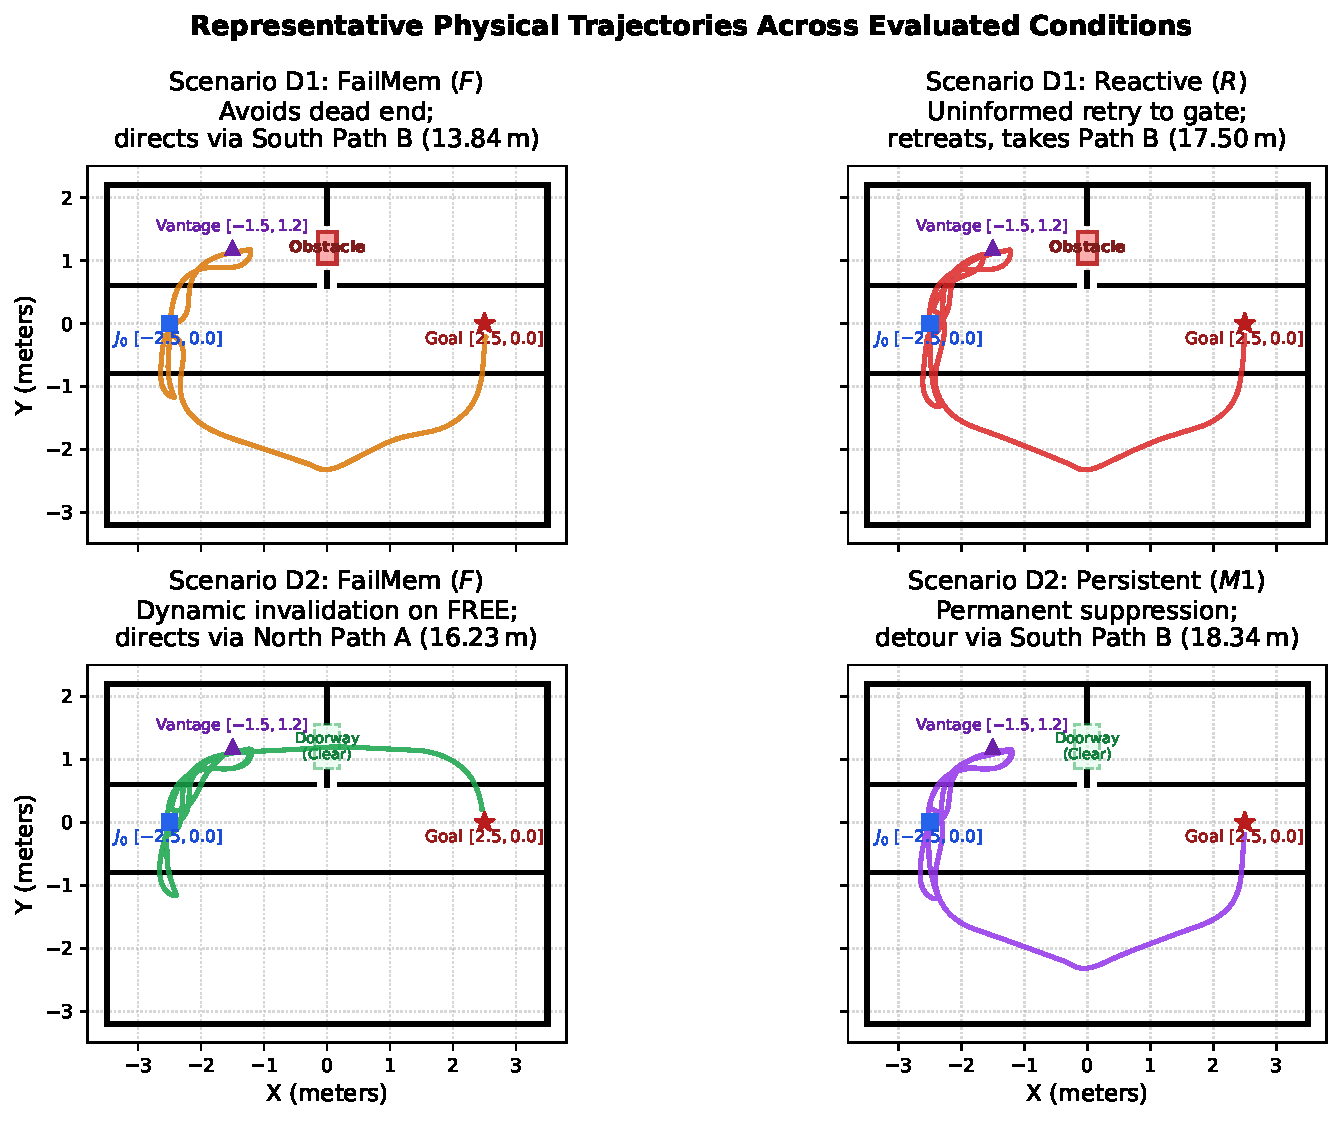
\includegraphics[width=\columnwidth]{figures/trajectories_map.pdf}
\caption{Representative Gazebo simulation trajectories across evaluated conditions.}
\label{fig:trajectories}
\end{figure}

\begin{enumerate}
    \item \textbf{Elimination of Redundant Dead-End Exploration ($F$ vs. $R$)}: In Scenario D1, FailMem ($F$) eliminates redundant entry into the blocked corridor ($0.0$ vs. $1.0$ dead ends), reducing total distance by $-18.5\%$ ($14.03\,\text{m}$ vs. $17.22\,\text{m}$) and simulation duration by $-22.3\%$ ($109.5\,\text{s}$ vs. $141.0\,\text{s}$) relative to Reactive $R$ (Table~\ref{tab:pairwise_contrasts}, Figure~\ref{fig:trajectories}). Reactive $R$'s dead-end traversal represents an unguided retry to the entrance waypoint, not collision.
    \item \textbf{Prevention of Detour Overhead ($F$ vs. $M1$)}: In Scenario D2, dynamic invalidation upon observing \texttt{FREE} unsuppresses Path A, reducing total distance by $\approx 11.0\%$ ($2.00\,\text{m}$, $16.25\,\text{m}$ vs. $18.25\,\text{m}$) relative to persistent suppression ($M1$). However, in the current 3-run exploratory evaluation, average total simulation duration showed no observed improvement and increased slightly by $\approx 1.5\%$ ($151.1\,\text{s}$ vs. $148.8\,\text{s}$, a sample mean difference of $+2.27\,\text{s}$). An independent three-phase trajectory time ledger analysis reveals the empirical source of this discrepancy: the $+2.27\,\text{s}$ full-episode duration sample mean difference was accrued predominantly during the \textbf{History Exploration Phase} ($t < T_{\text{history}}$), where FailMem took $100.00 \pm 7.72\,\text{s}$ vs. $M1$'s $97.53 \pm 2.12\,\text{s}$ (a $+2.47\,\text{s}$ exploration sample mean difference accrued prior to route dispatching). During the \textbf{Decision Phase} ($t \ge T_{\text{history}}$), execution durations between FailMem and $M1$ were virtually identical ($51.10 \pm 0.95\,\text{s}$ vs. $51.30 \pm 2.00\,\text{s}$, a difference of only $-0.20\,\text{s}$), indicating no observable end-to-end time advantage for Path A in this benchmark. An exploratory kinematic decomposition shows that along Path A, active moving time was shorter ($28.70 \pm 1.18\,\text{s}$ vs. $34.30 \pm 1.76\,\text{s}$ at default thresholds, a sample mean difference of $-5.60\,\text{s}$), reflecting shorter path length ($5.89\,\text{m}$ vs. $7.89\,\text{m}$), while stopped time was longer ($15.83 \pm 2.42\,\text{s}$ vs. $12.13 \pm 1.41\,\text{s}$, a sample mean difference of $+3.70\,\text{s}$), alongside independent doorway clearance settling window measurements ($6.97 \pm 0.06\,\text{s}$ vs. $4.60 \pm 0.00\,\text{s}$). Because component durations vary with discretization thresholds (active moving difference spans $-5.10\,\text{s}$ to $-6.80\,\text{s}$ and stationary difference spans $+3.10\,\text{s}$ to $+5.20\,\text{s}$ across linear velocity thresholds $0.03\text{--}0.08\,\text{m/s}$ in our sensitivity analysis, Supplementary Material Section S5), we report these as coarse-grained observational latencies rather than asserting an invariant physical mechanism.
    \item \textbf{Comparison with Spatial Caching in Static 2D Geometry ($F$ vs. $O$)}: In both D1 and D2, FailMem ($F$) and Spatial Cache ($O$) selected identical topological routes. Total distance differences ($+0.6\%$ in D1, $-0.9\%$ in D2) and total duration differences ($+0.7\%$ in D1, $+0.9\%$ in D2) remained under $1\%$. In the evaluated static 2D hallway layout, specific implementation, and run sample ($n=3$), no additional routing benefit of $F$ over $O$ was observed; this does not imply general lack of benefit across arbitrary domains or statistical equivalence. Notably, dynamic recovery upon obstacle removal is not exclusive to FailMem; spatial costmap caching ($O$) likewise updates its internal occupancy state and unblocks routes upon acquiring new sensory observations.
\end{enumerate}

\subsection{Feasibility Check for Action-Conditioned Navigation ($H_1$)}
To investigate whether action configurations (aligned $a_{\text{aligned}}$ vs. doorpost boundary-biased oblique $a_{\text{oblique}}$) create executability differences in an unobstructed doorway, a fixed 4-run feasibility check was conducted.

\begin{table*}[t]
\centering
\footnotesize
\caption{Exploratory Feasibility Results for Action-Conditioned Navigation Hypothesis $H_1$ ($n=4$).}
\label{tab:h1_feasibility}
\setlength{\tabcolsep}{3.0pt}
\begin{tabular*}{\textwidth}{@{\extracolsep{\fill}}llcccccccc@{}}
\toprule
Run Name & Profile & Target Goal & Perception & Nav2 Status & \shortstack{Nav2\\Time (s)} & \shortstack{Settling\\(s)} & \shortstack{Stability\\(s)} & \shortstack{Total\\Sim (s)} & Strict Arrival \\
\midrule
H1\_aligned\_run1 & act\_aligned & [1.50, 1.20] & FREE (23) & SUCCEEDED (4) & 13.4 & 3.0 & 2.4 & 18.8 & \shortstack{\textbf{False}\\\scriptsize($\omega_{\text{ang}}: 0.107 > 0.08$)} \\
H1\_aligned\_run2 & act\_aligned & [1.50, 1.20] & FREE (22) & SUCCEEDED (4) & 13.4 & 3.0 & 2.4 & 18.8 & \textbf{True} \\
H1\_oblique\_run1 & act\_oblique & [0.50, 0.88] & FREE (23) & SUCCEEDED (4) & 11.1 & 3.0 & 2.3 & 16.4 & \textbf{True} \\
H1\_oblique\_run2 & act\_oblique & [0.50, 0.88] & FREE (22) & SUCCEEDED (4) & 11.0 & 3.0 & 2.3 & 16.3 & \textbf{True} \\
\bottomrule
\end{tabular*}
\end{table*}


Table~\ref{tab:h1_feasibility} summarizes the feasibility trial outcomes. Nav2 returned \texttt{SUCCEEDED} (status code 4) in all 4/4 runs, and strict physical arrival was verified in 3/4 runs (\texttt{H1\_aligned\_run1} exceeded the angular velocity halt threshold during the stability window: $0.1068 > 0.08\,\text{rad/s}$). Nav2's \texttt{DWBLocalPlanner} navigated the passage without planner abortion across all runs.

\textbf{Decision \& Conclusion}: \emph{Nav2 returned success in 4/4 runs, with strict physical arrival verified in 3/4 runs; the candidate scenario did not establish the expected executability divergence. Exploration for this hypothesis was therefore stopped per protocol, which does not constitute a refutation of the general action-conditioned failure memory hypothesis.}
